\documentclass{article}

\usepackage{defines}

\begin{document}

\tickettitle{13}{Понятие векторного произведения векторов. Лемма о построении. Четыре~свойства~векторного~произведения.}

\define{векторного произведения векторов}

\begin{minipage}{0.6\linewidth}
	Векторное произведение $\vec{a}$ на $\vec{b}$ обозначается\\
	как $[\vec{a},\vec{b}]$ или $\vec{a}\times\vec{b}$:
	\begin{enumerate}
		\item{}$|\vec{a}\times\vec{b}|:=|\vec{a}||\vec{b}|\sin\angle(\vec{a},\vec{b})$
		\item{}$(\vec{a}\times\vec{b})\perp\vec{a}\land(\vec{a}\times\vec{b})\perp\vec{b}$
		\item{}$(\vec{a},\vec{b},\vec{c})$ --- правая тройка
	\end{enumerate}
\end{minipage}%
\begin{minipage}{0.4\linewidth}
	\centering
	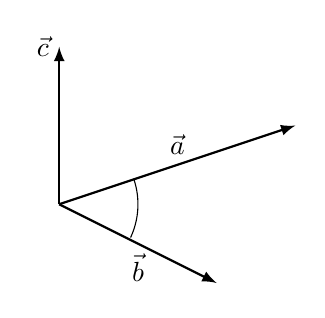
\begin{tikzpicture}
		\draw [-latex, thick] (0,0)--(3,1) node[midway, above] {$\vec{a}$};
		\draw [-latex, thick] (0,0)--(2,-1) node[midway, below] {$\vec{b}$};
		\draw [-latex, thick] (0,0)--(0,2) node[left] {$\vec{c}$};
		\draw [domain=-25:19] plot ({cos(\x)},{sin(\x)});
	\end{tikzpicture}
	\captionof{figure}{Векторное произведение}
\end{minipage}

\lemma[о построении]

\begin{minipage}{0.6\linewidth}
	$\vec{a}\nparallel\vec{e}\land|\vec{e}|=1$, тогда $[\vec{a},\vec{e}]=\lvec{OB}$ можно найти следущим образом:
	\begin{enumerate}
		\item{}Векторы $\vec{a}$ и $\vec{e}$ привести к общему началу $O$
		\item{}$\alpha:O\in\alpha\land\alpha\perp\vec{e}$
		\item{}$A':OA'\subset\alpha\land AA'\perp\alpha$ ($\lvec{OA}=\vec{a}$)
		\item{}$B:\angle A'OB=\pi/2\land OB\subset\alpha\land (\lvec{OA'},\vec{e},\lvec{OB})$ --- правая
	\end{enumerate}
\end{minipage}%
\begin{minipage}{0.4\linewidth}
	\centering
	\begin{tikzpicture}
		\coordinate (O) at (0,0) node [anchor=east] at (O) {$O$};
		\coordinate (Ap) at (2,-0.5) node [anchor=west] at (Ap) {$A'$};
		\coordinate (A) at (2,1) node [anchor=west] at (A) {$A$};
		\coordinate (B) at (-0.7,-1) node [anchor=east] at (B) {$B$};
		\draw [-latex] (O) -- (0,1.5) node [left] {$\vec{e}$};
		\draw [-latex] (O) -- (Ap);
		\draw [-latex] (O) -- (A) node[midway, above, xshift=1em, yshift=0.5em] {$\vec{a}$};
		\draw [-latex] (O) -- (B);
		\draw [dashed] (A) -- (Ap);
		\draw [domain=27:90] plot ({cos(\x)*0.4},{sin(\x)*0.4}) node[midway, xshift=1em, yshift=1.5em] {$\alpha$};
		\fill [opacity=0.3] ($1.2*(B)+1.2*(Ap)$)--($1.2*(B)-0.2*(Ap)$)--($-0.2*(B)-0.2*(Ap)$)--($-0.2*(B)+1.2*(Ap)$)--($1.2*(B)+1.2*(Ap)$)--cycle;
	\end{tikzpicture}
	\captionof{figure}{Лемма о построении}
\end{minipage}

\end{document}
